\documentclass[../../../../main.tex]{subfiles}

\begin{document}

\section*{京大理科 数学 1966 表紙・配点・概略}

\begin{itemize}
    \item 所要時間: 80分 / 150分
\end{itemize}

\subsection*{各問のメモ・解答概要}
\begin{enumerate}
    \item (1) $f(x) = x^3 + x - 8$ は単調増加で $f(1) < 0 < f(2)$ より $1 < x < 2$ に唯一の実根を持つ。(2) 背理法により根が有理数でないことを証明する。
    \item (i) 頂点が辺上にない場合は伸ばして面積を大きくできる。(ii) 平行四辺形の面積 $S$ に対し、最大面積は $\frac{1}{2}S$。 $S < 2$ のとき $\frac{1}{2}S < 1$ となり面積1の三角形は含まれない。
    \item 3本のテレビ塔の先端を結ぶ直線と平地の交点 A, B, C は、先端を含む平面と平地を含む平面の交線上にあるため一直線上にある。
    \item $0 < a \le \frac{1}{5}$ のとき $2-a$、$\frac{1}{5} \le a$ のとき $\sqrt{a^2 + \frac{9}{4}a + \frac{3}{2} + \frac{1}{4a}}$。
    \item 軌跡の領域を $u$ の範囲で分割して積分し、面積 $S = 2\left(a^3 - \frac{1}{a^3}\right)\log a$ を得る。
    \item 正 $n$ 角形の3頂点からなる鋭角三角形の個数。$n$ が奇数のとき $\frac{1}{24}n(n+1)(n-1)$、$n$ が偶数のとき $\frac{1}{24}n(n-2)(n-4)$。
\end{enumerate}

\newpage

\section*{第1問}

\noindent
[\textbf{解}]
\begin{enumerate}
    \item[(1)] $f(x) = x^3 + x - 8$ とおく。$f'(x) = 3x^2 + 1 > 0$ から、$f(x)$ は単調増加。
    これと $f(1) = -6$, $f(2) = 2$ より、$f(x) = 0$ は $1 < x < 2$ の区間に唯1つの実根を持つ。

    \item[(2)] 根を $\alpha$ とおくと
    \[
    \alpha^3 + \alpha - 8 = 0 \quad \dots \text{①}
    \]
    $\alpha$ が有理数だと仮定すると、$\alpha = \frac{b}{a}\ (a, b \in \mathbb{N})$ とおける。($(a, b)$ は互いに素) ①に代入して整理し
    \[
    b^3 = 8a^3 - b a^2 = a^2(8a - b)
    \]
    より、$b^3$ が $a^2$ で割り切れることが必要だが、$a, b$ は互いに素だからそのようなことはない。
    よって矛盾し、$\alpha \notin \mathbb{Q}$ である。
\end{enumerate}

\newpage

\section*{第2問}

\noindent
[\textbf{解}]
\begin{enumerate}
    \item[(i)] 3点 $P, Q, R$ が辺上にないとき、そのうちの1点をのばして、四角形の辺との交点に新たに点をとれば、より面積の大きい三角形ができるから、$P, Q, R$ は辺上にある。

    \begin{center}
    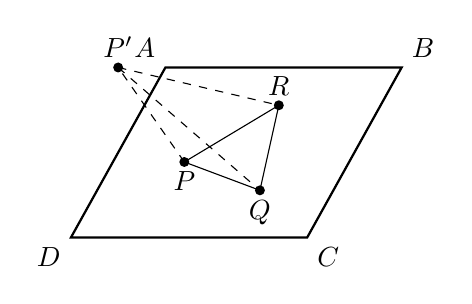
\begin{tikzpicture}[scale=1.2]
        \draw[thick] (0,0) node[below left]{$D$} -- (2.5,0) node[below right]{$C$} -- (3.5,1.8) node[above right]{$B$} -- (1,1.8) node[above left]{$A$} -- cycle;
        \coordinate (P) at (1.2,0.8);
        \coordinate (Q) at (2.0,0.5);
        \coordinate (R) at (2.2,1.4);
        \draw (P) -- (Q) -- (R) -- cycle;
        \fill (P) circle (1.5pt) node[below]{$P$};
        \fill (Q) circle (1.5pt) node[below]{$Q$};
        \fill (R) circle (1.5pt) node[above]{$R$};
        \coordinate (Pprime) at (0.5, 1.8);
        \draw[dashed] (P) -- (Pprime);
        \fill (Pprime) circle (1.5pt) node[above]{$P'$};
        \draw[dashed] (Pprime) -- (Q);
        \draw[dashed] (Pprime) -- (R);
    \end{tikzpicture}
    \end{center}

    \item[(ii)] $P, Q, R$ のうち、2点が同一辺上にある時は、その2点を頂点にした時が面積最大である $\dots$ ①

    \begin{center}
    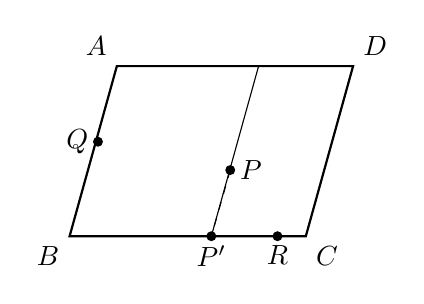
\begin{tikzpicture}[scale=1.2]
        \draw[thick] (0,0) node[below left]{$B$} -- (2.5,0) node[below right]{$C$} -- (3.0,1.8) node[above right]{$D$} -- (0.5,1.8) node[above left]{$A$} -- cycle;
        \draw (1.5,0) -- (2.0,1.8);
        \fill (0.3,1.0) circle (1.5pt) node[left]{$Q$};
        \fill (1.7,0.7) circle (1.5pt) node[right]{$P$};
        \fill (1.5,0) circle (1.5pt) node[below]{$P'$};
        \fill (2.2,0) circle (1.5pt) node[below]{$R$};
        \draw[dashed] (1.7,0.7) -- (1.5,0);
    \end{tikzpicture}
    \end{center}

    又、3点とも異なる辺上にある時、対称性からそれを図ようにおく。
    $P$ を通り $AB$ に平行な直線と $BC$ の交点を $P'$ とする。まず $P, R$ を固定。

    \begin{enumerate}
        \item[$1^\circ$] $R$ が $BP'$ 上にある時\\
        $PR$ を底辺とみて、$Q=A$ の時 $\triangle PQR$ は最大。さらに、次に $P$ をうごかして、$P=D$ の時 $\triangle PQR$ は最大値 $\frac{1}{2}\square ABCD$ をとる。

        \item[$2^\circ$] $R$ が $P'C$ 上にある時\\
        同様にして $Q=B, R=C$ の時 $\triangle PQR$ は最大値 $\frac{1}{2}\square ABCD$ をとる。
    \end{enumerate}

    この時の最大値も同じく $\frac{1}{2}\square ABCD$ だから、以上あわせて題意は示された。

    \item[(iii)] (i)から、面積 $S$ の平行四辺形の内に入る三角形の最大面積が $\frac{1}{2}S$ だから、$S < 2$ の時、$\frac{1}{2}S < 1$ となり、面積 1 の三角形は入らない。
\end{enumerate}

\newpage

\section*{第3問}

\noindent
[\textbf{解}] 3本のテレビ塔を $P, Q, R$ としてその高さを $p, q, r\ (p < q < r)$ とする。等号が全て成立することはない。さて、3点 $A, B, C$ は $P, Q$ の先端を結ぶ直線と平地の交点、$Q, R$ の、 $R, P$ のとおいてよい。

すると、$A, B, C$ はテレビ塔の3先端を含む平面内かつ平地を含む平面内にある。2平面が交わる時 その交線は直線となるから、3点 $A, B, C$ は一直線上にある。

\newpage

\section*{第4問}

\noindent
[\textbf{解}] 右図のような座標平面を考える。

\begin{center}
\begin{tikzpicture}[scale=1.5]
    \draw[->] (-0.5,0) -- (3,0) node[below]{$x$};
    \draw[->] (0,-1) -- (0,1.5) node[left]{$y$};
    \fill (0,0) circle (1.5pt) node[below left]{$A$};
    \fill (1.5,0) circle (1.5pt) node[below]{$B$};
    \node at (0.75,-0.15) {$a$};
    \draw[domain=0:2.5,smooth,variable=\x,thick] plot ({\x}, {-0.4*sin(\x*180)});
\end{tikzpicture}
\end{center}

\noindent
すると $0 \le \theta < 2\pi$ として
\[
\vec{AP} = \begin{pmatrix} \cos 2\theta \\ \sin 2\theta \end{pmatrix}, \quad
\vec{AQ} = \begin{pmatrix} a \\ 0 \end{pmatrix} + \begin{pmatrix} \cos(-\theta) \\ \sin(-\theta) \end{pmatrix}
\]
とおけるから
\[
\vec{PQ} = \begin{pmatrix} a + \cos\theta - \cos 2\theta \\ -\sin\theta - \sin 2\theta \end{pmatrix}
\]
$|\vec{PQ}| \ge 0$ から、$|\vec{PQ}|^2$ が最大の時、$|\vec{PQ}|$ も最大。以下 $\cos\theta = c, \sin\theta = s$ と略記して、
\begin{align*}
|\vec{PQ}|^2 &= \{ a + c - (2c^2 - 1) \}^2 + (-s - 2cs)^2 \\
&= (-2c^2 + c + a + 1)^2 + s^2(1 + 2c)^2 \\
&= 4c^4 - 4c^3 - (4a + 3)c^2 + 2(a + 1)c + (a + 1)^2 + (1 - c^2)(4c^2 + 4c + 1) \\
&= -4ac^2 + 2(a - 1)c + (a^2 + 2a + 2) \equiv f(c)
\end{align*}
以下 $f(c)$ の最大値を求める。$a > 0$ に注意して、軸の大きさで場合分けする。

\begin{center}
\begin{tikzpicture}[scale=1.5]
    \draw[->] (-1.2,0) -- (1.5,0) node[right]{$c$};
    \draw[->] (0,-0.5) -- (0,1.5);
    \draw (-1, -0.05) -- (-1, 0.05) node[above]{$-1$};
    \draw (1, -0.05) -- (1, 0.05) node[above]{$1$};
    \draw[dashed] (0.3,-0.3) -- (0.3,1.2) node[above]{軸 $c = \frac{a-1}{4a}$};
    \draw[thick, domain=-1:1] plot ({\x}, {-0.8*(\x-0.3)*(\x-0.3) + 1});
\end{tikzpicture}
\end{center}

\begin{enumerate}
    \item[$1^\circ$] $0 < a \le \frac{1}{5}$ の時
    \[
    \max f(c) = f(-1) = (a - 2)^2
    \]
    \item[$2^\circ$] $\frac{1}{5} \le a$ の時
    \[
    \max f(c) = f\left(\frac{a-1}{4a}\right) = a^2 + \frac{9}{4}a + \frac{3}{2} + \frac{1}{4a}
    \]
\end{enumerate}
以上から、
\[
\begin{cases}
0 < a \le \frac{1}{5} \text{の時} & 2 - a \\
\frac{1}{5} \le a \text{の時} & \sqrt{a^2 + \frac{9}{4}a + \frac{3}{2} + \frac{1}{4a}}
\end{cases}
\]

\newpage

\section*{第5問}

\noindent
[\textbf{解}] $P$ が $ABCD$ を1周する時、
\[
\begin{cases}
AB \text{上} \dots y = 1, -1 \le x \le 1 & \dots \text{①} \\
BC \text{上} \dots x = -1, -1 \le y \le 1 & \dots \text{②} \\
CD \text{上} \dots y = -1, -1 \le x \le 1 & \dots \text{③} \\
DA \text{上} \dots x = 1, -1 \le y \le 1 & \dots \text{④}
\end{cases}
\]
である。従って、$Q(u, v)$ のキセキは以下。($a > 1$ に注意)

\begin{enumerate}
    \item[$1^\circ$] ①の時
    \[
    u = a \cdot a^x, \quad v = \frac{1}{a} \cdot a^{2x} \quad (-1 \le x \le 1)
    \]
    から、
    \[
    v = \frac{1}{a^3} u^2 \quad (1 \le u \le a^2)
    \]

    \item[$2^\circ$] ②の時
    \[
    u = \frac{1}{a} \cdot a^y, \quad v = \frac{1}{a^2} \cdot a^{-y} \quad (-1 \le y \le 1)
    \]
    から
    \[
    v = \frac{1}{a^3} \frac{1}{u} \quad \left(\frac{1}{a^2} \le u \le 1\right)
    \]

    \item[$3^\circ$] ③の時
    \[
    u = \frac{1}{a} \cdot a^x, \quad v = a \cdot a^{2x} \quad (-1 \le x \le 1)
    \]
    から
    \[
    v = a^3 u^2 \quad \left(\frac{1}{a^2} \le u \le 1\right)
    \]

    \item[$4^\circ$] ④の時
    \[
    u = a \cdot a^y, \quad v = a^2 \cdot a^{-y} \quad (-1 \le y \le 1)
    \]
    から
    \[
    v = a^3 \frac{1}{u} \quad (1 \le u \le a^2)
    \]
\end{enumerate}

図示して右図のようになる。求める面積 $S$ のうち $\frac{1}{a^2} \le u \le 1$ のものを $S_1$, $1 \le u \le a^2$ のものを $S_2$ として、
\[
S = S_1 + S_2 \quad \dots \text{⑤}
\]

\begin{center}
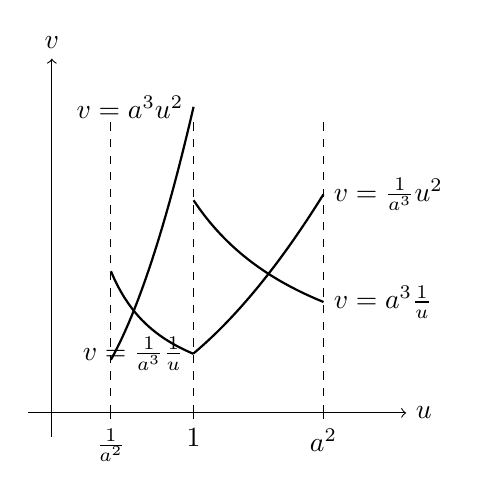
\begin{tikzpicture}[scale=1.5]
    \draw[->] (-0.2,0) -- (3,0) node[right]{$u$};
    \draw[->] (0,-0.2) -- (0,3) node[above]{$v$};
    \draw (0.5,0.05) -- (0.5,-0.05) node[below]{$\frac{1}{a^2}$};
    \draw (1.2,0.05) -- (1.2,-0.05) node[below]{$1$};
    \draw (2.3,0.05) -- (2.3,-0.05) node[below]{$a^2$};
    
    \draw[thick, domain=0.5:1.2] plot ({\x}, {1.8*\x*\x}) node[left]{$v=a^3 u^2$};
    \draw[thick, domain=0.5:1.2] plot ({\x}, {0.6/\x}) node[left]{$v=\frac{1}{a^3}\frac{1}{u}$};
    \draw[thick, domain=1.2:2.3] plot ({\x}, {2.16/\x}) node[right]{$v=a^3\frac{1}{u}$};
    \draw[thick, domain=1.2:2.3] plot ({\x}, {0.35*\x*\x}) node[right]{$v=\frac{1}{a^3}u^2$};
    \draw[dashed] (0.5,0) -- (0.5,2.5);
    \draw[dashed] (1.2,0) -- (1.2,2.5);
    \draw[dashed] (2.3,0) -- (2.3,2.5);
\end{tikzpicture}
\end{center}

\begin{align*}
S_1 &= \int_{\frac{1}{a^2}}^1 \left( a^3 u^2 - \frac{1}{a^3 u} \right) du \\
&= \left[ \frac{a^3}{3} u^3 - \frac{1}{a^3} \log u \right]_{\frac{1}{a^2}}^1 \\
&= \frac{a^3}{3} - \left( \frac{1}{3a^3} + \frac{2}{a^3} \log a \right) \\
&= \frac{1}{3}a^3 - \frac{1}{3a^3} - \frac{2}{a^3}\log a \\[10pt]
S_2 &= \int_1^{a^2} \left( a^3 \frac{1}{u} - \frac{1}{a^3} u^2 \right) du \\
&= \left[ a^3 \log u - \frac{1}{3a^3} u^3 \right]_1^{a^2} \\
&= 2a^3 \log a - \frac{1}{3}a^3 + \frac{1}{3a^3}
\end{align*}
⑤へ代入して、
\[
S = 2\left(a^3 - \frac{1}{a^3}\right)\log a
\]

\newpage

\section*{第6問}

\noindent
[\textbf{解}]
\begin{enumerate}
    \item[(1)] $n$ 個の頂点の中から3つ選べば三角形が1つ対応するので、
    \[
    _n\mathrm{C}_3 = \frac{1}{6}n(n-1)(n-2)
    \]

    \item[(2)] (1)から、鈍角三角形、直角三角形のものをのぞけばよい。

    \begin{enumerate}
        \item[$1^\circ$] $n = 2k\ (k \in \mathbb{N}_{\ge 2})$ の時\\
        1つの頂点を $A_1$ とする。$A_1 A_{k+1}$ が外接円の直径だから、鈍角をつくるには右図の分領域から2点を考えればよく、
        \[
        \begin{cases}
        k \ge 3 \text{のとき} & _{k-1}\mathrm{C}_2 \text{通り} \\
        k \le 2 \text{の時} & 0 \text{通り}
        \end{cases}
        \]
        1つの頂点が他にある場合と重複を考えて、
        \[
        \begin{cases}
        k \ge 3 \text{の時} & 2k \cdot _{k-1}\mathrm{C}_2 / 2 = k(k-1)(k-2) \text{通り} \\
        k \le 2 \text{の時} & 0 \text{通り}
        \end{cases}
        \]

        \begin{center}
        \begin{tikzpicture}[scale=1.2]
            \draw (0,0) circle (1.2);
            \fill (0,1.2) circle (1.5pt) node[above]{$A_1$};
            \fill (0,-1.2) circle (1.5pt) node[below]{$A_{k+1}$};
            \draw[dashed] (0,1.2) -- (0,-1.2);
            \draw[thick] (0.1,1.1) arc (80:-80:1.1);
            \draw[thick] (-0.1,1.1) arc (100:260:1.1);
            \node at (0.5,0.5) {$2\text{つ}$};
        \end{tikzpicture}
        \end{center}

        一方、直角三角形は1つの直径となる辺に対し、のこり1つの辺のえらび方が $2k-2$ 通りあるから、
        \[
        k(2k-2) \text{通り}
        \]

        \item[$2^\circ$] $n = 2k-1$ の時\\
        1°と同様に考える。1つの頂点を $A_1$ に固定した時、鈍角三角形は
        \[
        \begin{cases}
        k \ge 3 \text{のとき} & _{k-1}\mathrm{C}_2 \text{通り} \\
        k \le 2 \text{の時} & 0 \text{通り}
        \end{cases}
        \]
        だから、あわせて
        \[
        \begin{cases}
        k \ge 3 \text{の時} & (2k-1) \cdot _{k-1}\mathrm{C}_2 \text{通り} \\
        k = 2 \text{の時} & 0 \text{通り}
        \end{cases}
        \]
        直角三角形は存在しない。

        \begin{center}
        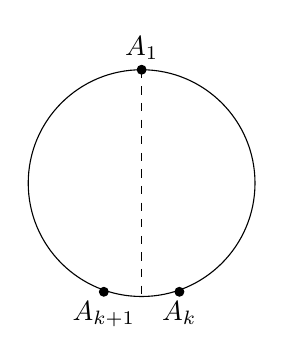
\begin{tikzpicture}[scale=1.2]
            \draw (0,0) circle (1.2);
            \fill (0,1.2) circle (1.5pt) node[above]{$A_1$};
            \fill (-0.4,-1.15) circle (1.5pt) node[below]{$A_{k+1}$};
            \fill (0.4,-1.15) circle (1.5pt) node[below]{$A_k$};
            \draw[dashed] (0,1.2) -- (0,-1.2);
        \end{tikzpicture}
        \end{center}
    \end{enumerate}

    以上から、求める数は $n=3$ の時 1、$n=4$ の時 0 で、$n \ge 5$ の時
    \[
    n \in \text{even の時}: \quad \frac{1}{6}n(n-1)(n-2) - \frac{n}{2}\left(\frac{n}{2}-1\right)\left(\frac{n}{2}-2\right) - \frac{n}{2}(n-2) = \frac{1}{24}n(n-2)(n-4)
    \]
    \[
    n \in \text{odd の時}: \quad \frac{1}{6}n(n-1)(n-2) - \frac{1}{2}n\left(\frac{n-1}{2}\right)\left(\frac{n-3}{2}\right) = \frac{1}{24}n(n+1)(n-1)
    \]
    これらは $n=3, 4$ でも成立するから
    \[
    \begin{cases}
    n \in \text{odd} & \frac{1}{24}n(n+1)(n-1) \\
    n \in \text{even} & \frac{1}{24}n(n-2)(n-4)
    \end{cases}
    \]
    である。
\end{enumerate}

\end{document}
